\subsection{Higgs mechanism and Electroweak symmetry breaking}
\label{symbreaking}

As shown in previous subsection, the Lagrangian $L_{gauge}$ does not involve any mass term due to the requirement of gauge invariance.
So all the W and B bosons should be massless. But experimental observations show that the gauge bosons are massive.
Therefore, the gauge invariance must be broken spontaneously.
The Higgs field is introduced to break the $SU(2)_{L} \times U(1)_{Y}$ symmetry and
guage bosons and fermions can interact with Higgs filed to acquire their masses.
And this specific process is named \textit{Higgs mechanism} in SM.

The Higgs field $\phi$ is a doublet and can be written in a Hermitian basis as
\begin{equation}
	\phi = \binom{\phi^{+}}{\phi^{0}} = \frac{1}{\sqrt{2}} \binom{\phi_{1} - i\phi_{2}}{\phi_{3} - i\phi_{4}}
\end{equation}
where $\phi_{i} = \phi_{i}^{+}$ stand for four Hermitian field. 
In this new basis, the Higgs potential in Eq.~\ref{eq:Vhiggs} can be expressed as:
\begin{equation}
	V(\phi) = \frac{1}{2}\mu^{2}\left(\sum_{i=1}^{4}\phi_{i}^{2}\right) + \frac{1}{4}\lambda\left(\sum_{i=1}^{4}\phi_{i}^{2}\right)^{2}
\end{equation}
To simplify the situation, the axis in this four-dimensional space can be choosen to satisfied
~$\left<0\left| \phi_{i} \right|0\right> = 0$ for $i = 1, 2, 4$, and $<0\left| \phi_{3} \right|0> = v$. Thus,
\begin{equation}
	V(\phi) \rightarrow V(v) = \frac{1}{2}\mu^{2}v^{2} + \frac{1}{4}\lambda v^{4}
\end{equation}
The minimization of this potential depends on the sign of $\mu^{2}$ as shown in figure~\ref{fig:C2_Higgs_potential}.
When $\mu^{2} > 0$ the minimum occurs at $v = 0$, namely the vacuum is empty space and $SU(2)_{L} \times U(1)_{Y}$ symmetry is unbroken.
In the case of $\mu^{2} < 0$, the $v = 0$ symmetric point is no longer stable and the minimum occurs at nonzero value of 
$v = \left( -\mu^{2}/\lambda\right)^{1/2}$ which breaks the $SU(2)_{L} \times U(1)_{Y}$ symmetry.
\begin{figure}[!htb]
  \centering
  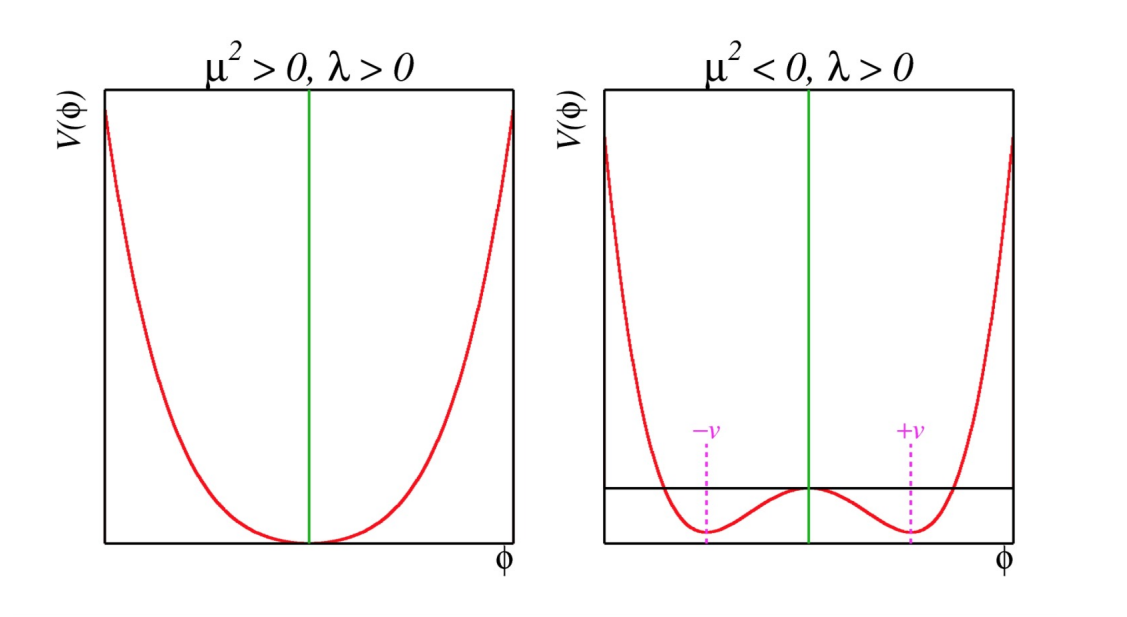
\includegraphics[width=0.7\textwidth]{figures/Theory/Vhiggs.png}
  \caption{Higgs potential $V(\phi)$ with $\mu^{2}>0$ (left) and $\mu^{2}<0$ (right).}
  \label{fig:C2_Higgs_potential}
\end{figure}
Thus, the classical vacuum $\phi_{0}$ of Higgs doublet can be expressed by
\begin{equation}
	\phi_{0} = \frac{1}{\sqrt{2}}\binom{0}{v}
\end{equation}
And to quantize around the classical vacuum in a general form:
\begin{equation}
	\phi = \frac{1}{\sqrt{2}} \binom{0}{v+H}
\end{equation}
Where H is a Hermitian field for physical Higgs scalar.
In this guage, the Lagrangian $L_{Higgs}$ in Eq.~\ref{eq:Lhiggs} takes a simple form
\begin{equation}
\begin{split} \label{eq:Lhiggs2}
	L_{Higgs} & = \left(D^{\mu}\phi\right)^{\dagger}D_{\mu}\phi - V(\phi) \\
	& = M_{W}^{2}W^{\mu+}W_{\mu}^{-}\left(1+\frac{H}{\nu}\right)^{2} + \frac{1}{2}M_{Z}^{2}Z^{\mu}Z_{\mu}\left(1+\frac{H}{\nu}\right)^{2} \\ 
        &   + \frac{1}{2}\left(\partial_{\mu}H\right)^{2} - V(\phi)
\end{split}
\end{equation}
where the W and Z fields are
\begin{equation}
\begin{split}
	& W^{\pm} = \frac{1}{\sqrt{2}} \left(W^{1} \mp iW^{2}\right) \\
	& Z = - sin\theta_{W}B + cos\theta_{W}W^{3}
\end{split}
\end{equation}
Therefore, in Eq.~\ref{eq:Lhiggs2} spontaneous symmetry breaking brings out masses for the W and Z gauge bosons
\begin{equation}
\begin{split}
	& M_{W} = \frac{gv}{2} \\
	& M_{Z} = \sqrt{g^{2} + g'^{2}} \frac{v}{2} = \frac{M_{W}}{cos\theta_{W}}
\end{split}
\end{equation}
where $\theta_{W}$ is the weak angle defined as
\begin{equation}
	sin\theta_{W} = \frac{g'}{\sqrt{g^{2} + g'^{2}}} \qquad cos\theta_{W} = \frac{g}{\sqrt{g^{2} + g'^{2}}} \qquad tan\theta_{W} = \frac{g'}{g}
\end{equation}
Then another gauge boson photon remains massless with the field of
\begin{equation}
	A = cos\theta_{W}B + sin\theta_{W}W^{3}
\end{equation}

After the symmetry breaking, the Higgs potential in unitary gauge can be written into
\begin{equation}
	V(\phi) = -\frac{\mu^{4}}{4\lambda} - \mu^{4}H^{2} + \lambda\nu H^{3} + \frac{\lambda}{4}H^{4}
\end{equation}
The first term in $V$ is a constant, while the second term denotes a (tree-level) mass of Higgs boson
\begin{equation}
	M_{H} = \sqrt{-2\mu^{2}} = \sqrt{2\lambda}v
\end{equation}
Due to the unknown of  quartic Higgs coupling $\lambda$, the Higgs mass is not predicted.
The third and fourth terms in Higgs potential $V$ denote the induced cubic and quartic interactions of the Higgs scalar.

Through the Higgs mechanism, fermions can also acquire their masses.
In the unitary gauge, Yukawa Lagrangian ($L_{Yukawa}$) can be written as a simple form of \cite{Pich:2015lkh}
\begin{equation}
	L_{Yukawa} = -\left(1+\frac{H}{v}\right) \left(m_{d}\bar{d}d + m_{u}\bar{u}u + m_{l}\bar{l}l\right)
\end{equation}
in which $m_{f} = \frac{y_{f}v}{\sqrt{2}}$ for $f = d, u, l$.
